\begin{document}

\subsection{Summer Experience in Science and Engineering for Youth}

\outreachEntry{07/14/19-07/19/19}{Connect}{Sarah}{

\textbf{Summary:} Summer Experience in Science and Engineering for Youth [SESEY] is a camp held at Oregon State University in Corvallis, Oregon, for a week. The camp is run by current Associate Professor of Chemical Engineering in the School of Chemical, Biological, and Environmental Engineering, Dr.Skip Rochefort. During the week, the camp attendees stay in dorm rooms and eat at the dining halls to additionally get an experience of what college might be like. For the most part, the attendees are from the West Coast but there were some from places like El Salvador, Hawaii, and Louisiana. During the camp, we also got sessions where we learned about different engineering majors and careers, college life, choosing a college, and much more. We also were fortunate to get a college tour of parts of University of Oregon in Eugene, Oregon where we got to see the Center for Advanced Materials Characterization which is where they make and produce semi conductors that would later be used in anything from phones to computers to GPS's. 
\\\\
The main focus of the camp though was to have Lab Projects where the camp attendees would be separated and put into groups to do different lab groups. Each lab group consisted of about 2-5 students, a faculty member, and student mentor who helped guide and teach the attendees more about their assigned topic. At the end of the week, the goal was to have a poster summarizing everything you did and learned.
\\\\
My topic was Robotics for Multidisciplinary Learning in which me and 3 other students tested a course that our student mentor, Megan McCormick, had created. We tested an ECE 111 Class course created by our student mentor to check for errors, confusions, and anything that may make the course difficult to complete. We started out by completing the different tutorials that would be needed to complete the labs. We tested them on PCs (Windows XP) and a MacBook. We provided feedback after every tutorial and lab, so they knew what to adjust for the class. The ending goal for this course was to create a mini robot using the skills we had learned or revisited over the past 2 days.
\\\\
\textbf{Impact: }SESEY helped me be more informed about what it would be like to take Electrical Computer Engineering course would be like and also helped me find out a little bit if I was actually interested in Electrical Computer Engineering. It was also really beneficial to listen to the talks from a college professor about what the application people are actually interested in and what they look at when they're going through applications. It was also interesting to talk and ask questions to the camp counselors who go to Oregon State to see what college life is like there. It was also beneficial to sleep for a week in the dorms to see what Weatherford Dorms were like. It was also cool and interesting to compare the University of Oregon campus with the Oregon State Campus and to see the engineering and semi conductor stuff at both colleges.

}
\begin{center}
    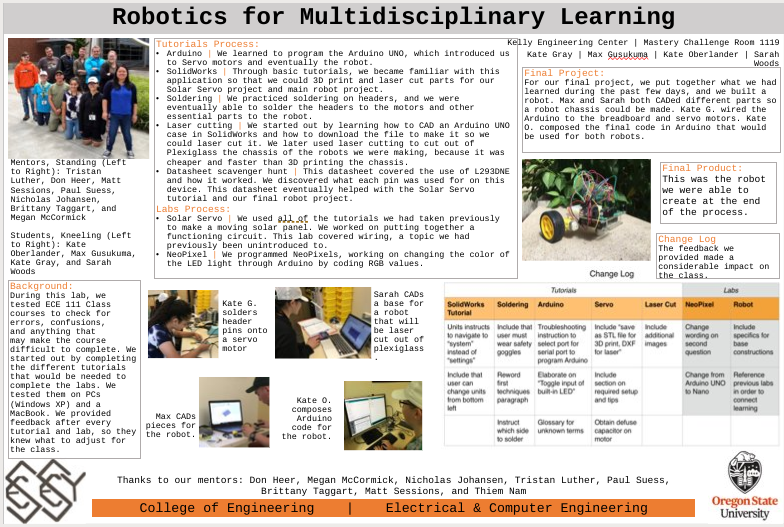
\includegraphics[width=.75\textwidth]{OutreachImages/SESEY(II).png}\\
    The completed poster
    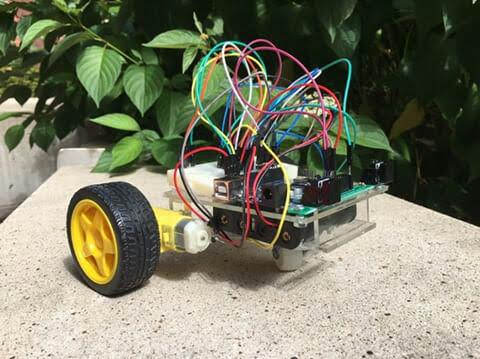
\includegraphics[width=.75\textwidth]{OutreachImages/SESEY(I).jpeg}\\
    The completed robot
\end{center}

\end{document}